\documentclass[11pt]{article}
\usepackage{amsmath, amssymb}
\usepackage{geometry}
\usepackage{hyperref}
\usepackage{booktabs}
\usepackage{xcolor}
\usepackage{tikz}
\usetikzlibrary{arrows.meta, positioning, decorations.pathreplacing, calc}
\geometry{margin=2.5cm}

\definecolor{isingblue}{RGB}{45,105,170}
\definecolor{isingred}{RGB}{190,70,55}
\definecolor{kitaevgreen}{RGB}{40,135,100}
\definecolor{linkgray}{RGB}{90,90,90}
\definecolor{softgray}{RGB}{245,245,245}

\newcommand{\ket}[1]{|#1\rangle}
\newcommand{\bra}[1]{\langle#1|}
\newcommand{\up}{\uparrow}
\newcommand{\down}{\downarrow}

\title{Antiferromagnetic Ising Model vs the Kitaev-Chain Qubit Hamiltonian}
\author{Seminar notes}
\date{\today}

\begin{document}
\maketitle

\section{The Short Version}

At the sweet spot $t=\Delta$, $\mu=0$, the Jordan-Wigner image of the Kitaev
chain is
\begin{equation}
  H_K = t\sum_{j=0}^{L-2}Y_jY_{j+1}.
\end{equation}
Since $t>0$, each bond prefers opposite $Y$ eigenvalues, so algebraically this
looks like an antiferromagnetic Ising chain written in the $Y$ basis.

The important difference is physical meaning. In the antiferromagnetic Ising
model, the spins are the physical ordered variables and the two ground states
are distinguished by local staggered magnetization. In the Kitaev chain, the
qubits are a Jordan-Wigner encoding of fermions, and the important degeneracy
is the occupation of a non-local edge fermion made from two Majorana modes. In
the original fermionic language, the order is not a local staggered
magnetization; it is detected by parity, edge degeneracy, and non-local string
operators.

\begin{figure}[h]
\centering
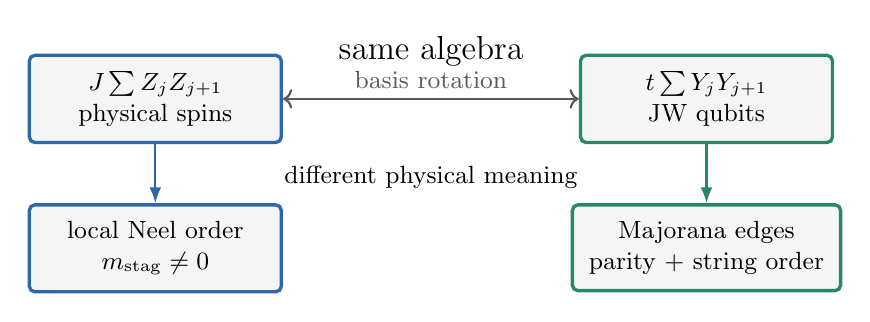
\begin{tikzpicture}[
  font=\small,
  box/.style={draw, rounded corners=2pt, fill=softgray, align=center,
    inner sep=6pt, minimum width=3.2cm, minimum height=1.0cm},
  afmbox/.style={box, draw=isingblue, very thick},
  kitbox/.style={box, draw=kitaevgreen, very thick},
  arr/.style={-{Latex[length=2mm]}, thick}
]
  \node[afmbox] (afmH) at (0,0) {$J\sum Z_jZ_{j+1}$\\ physical spins};
  \node[afmbox, below=0.75cm of afmH] (afmO) {local Neel order\\ $m_{\mathrm{stag}}\neq0$};
  \node[kitbox] (kitH) at (7.0,0) {$t\sum Y_jY_{j+1}$\\ JW qubits};
  \node[kitbox, below=0.75cm of kitH] (kitO) {Majorana edges\\ parity + string order};
  \draw[arr, isingblue] (afmH) -- (afmO);
  \draw[arr, kitaevgreen] (kitH) -- (kitO);
  \draw[<->, thick, linkgray] (afmH) -- node[above, font=\small] {basis rotation} (kitH);
  \node[align=center, font=\large] at (3.5,0.6) {same algebra};
  \node[align=center, font=\small] at (3.5,-1) {different physical meaning};
\end{tikzpicture}
\caption{The central point: the sweet-spot qubit Hamiltonian has an Ising-like
algebraic form, but the variables and diagnostics represent different physics.}
\label{fig:concept-map}
\end{figure}

\section{Spin Variables and Pauli Operators}

The classical Ising model starts with a two-valued spin variable at every site:
\begin{equation}
  S_j=\pm 1.
\end{equation}
For a quantum spin-$\frac{1}{2}$ degree of freedom, the local Hilbert space is
two-dimensional. We choose the $Z$ basis
\begin{equation}
  \ket{\up}_j=\ket{0}_j,
  \qquad
  \ket{\down}_j=\ket{1}_j,
\end{equation}
with
\begin{equation}
  Z_j\ket{\up}_j=+\ket{\up}_j,
  \qquad
  Z_j\ket{\down}_j=-\ket{\down}_j.
\end{equation}
Thus the classical value $S_j$ is represented by the eigenvalue of the Pauli
operator $Z_j$:
\begin{equation}
  S_j \longleftrightarrow Z_j.
\end{equation}

If one uses physical spin operators, they are related to Pauli matrices by
\begin{equation}
  S_j^\alpha=\frac{\hbar}{2}\sigma_j^\alpha,
  \qquad \alpha=x,y,z.
\end{equation}
In quantum-information notation we usually absorb the factors of $\hbar/2$
into the coupling constants and write Hamiltonians directly using Pauli
operators $X,Y,Z$.

\section{Antiferromagnetic Ising Hamiltonian}

\subsection{Classical and quantum forms}

The nearest-neighbor antiferromagnetic Ising chain is
\begin{equation}
  H_{\mathrm{AFM}}
  = J\sum_{j=0}^{L-2}Z_jZ_{j+1},
  \qquad J>0.
  \label{eq:afm-ising}
\end{equation}
The sign $J>0$ means that an aligned bond has positive energy and an
anti-aligned bond has negative energy.

For one bond,
\begin{equation}
  H_{j,j+1}=JZ_jZ_{j+1}.
\end{equation}
The four two-spin basis states are eigenstates:
\begin{center}
\begin{tabular}{ccc}
\toprule
State & $Z_jZ_{j+1}$ eigenvalue & Bond energy \\
\midrule
$\ket{\up\up}$ & $+1$ & $+J$ \\
$\ket{\down\down}$ & $+1$ & $+J$ \\
$\ket{\up\down}$ & $-1$ & $-J$ \\
$\ket{\down\up}$ & $-1$ & $-J$ \\
\bottomrule
\end{tabular}
\end{center}
For $J>0$, the low-energy bond states are therefore
\begin{equation}
  \ket{\up\down},
  \qquad
  \ket{\down\up}.
\end{equation}

\subsection{Ground states and energies}

Because all $Z_jZ_{j+1}$ terms commute, every product state in the $Z$ basis is
an eigenstate of Eq.~\eqref{eq:afm-ising}. If a configuration has
$N_{\mathrm{same}}$ aligned bonds and $N_{\mathrm{opp}}$ anti-aligned bonds,
then
\begin{equation}
  E=J(N_{\mathrm{same}}-N_{\mathrm{opp}}),
  \qquad
  N_{\mathrm{same}}+N_{\mathrm{opp}}=L-1.
\end{equation}
On an open chain, the minimum energy is obtained by making every bond
anti-aligned:
\begin{equation}
  E_0=-J(L-1).
\end{equation}
There are two such ground states:
\begin{equation}
  \ket{N_1}=\ket{\up\down\up\down\cdots},
  \qquad
  \ket{N_2}=\ket{\down\up\down\up\cdots}.
  \label{eq:neel-states}
\end{equation}
These are the two Neel states. A local defect where one bond fails to alternate
changes that bond energy from $-J$ to $+J$, so one bad bond costs
\begin{equation}
  \Delta E_{\mathrm{bad\ bond}}=2J.
\end{equation}
These local defects are domain walls in the antiferromagnetic order.

\begin{figure}[h]
\centering
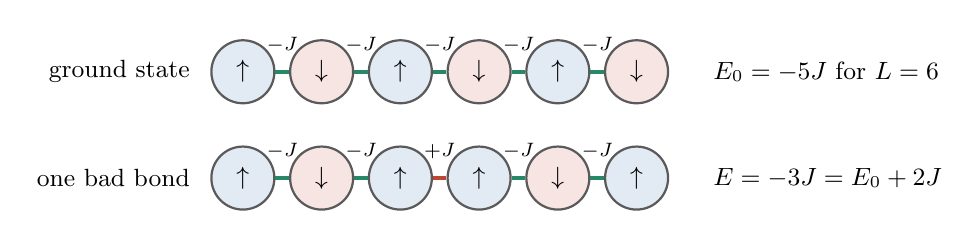
\begin{tikzpicture}[
  font=\small,
  spin/.style={circle, draw=linkgray, thick, minimum size=8mm, inner sep=0pt},
  good/.style={line width=1.3pt, draw=kitaevgreen},
  bad/.style={line width=1.3pt, draw=isingred}
]
  \node[anchor=east] at (-0.55,0) {ground state};
  \foreach \i/\lab/\clr in {0/{\up}/{isingblue!14},1/{\down}/{isingred!14},2/{\up}/{isingblue!14},3/{\down}/{isingred!14},4/{\up}/{isingblue!14},5/{\down}/{isingred!14}} {
    \node[spin, fill=\clr] (g\i) at (\i*1.0,0) {$\lab$};
  }
  \foreach \i/\j in {0/1,1/2,2/3,3/4,4/5} {
    \draw[good] (g\i.east) -- node[above=3pt, font=\scriptsize] {$-J$} (g\j.west);
  }
  \node[anchor=west] at (5.85,0) {$E_0=-5J$ for $L=6$};

  \node[anchor=east] at (-0.55,-1.35) {one bad bond};
  \foreach \i/\lab/\clr in {0/{\up}/{isingblue!14},1/{\down}/{isingred!14},2/{\up}/{isingblue!14},3/{\up}/{isingblue!14},4/{\down}/{isingred!14},5/{\up}/{isingblue!14}} {
    \node[spin, fill=\clr] (d\i) at (\i*1.0,-1.35) {$\lab$};
  }
  \foreach \i/\j in {0/1,1/2,3/4,4/5} {
    \draw[good] (d\i.east) -- node[above=3pt, font=\scriptsize] {$-J$} (d\j.west);
  }
  \draw[bad] (d2.east) -- node[above=3pt, font=\scriptsize] {$+J$} (d3.west);
  \node[anchor=west] at (5.85,-1.35) {$E=-3J=E_0+2J$};
\end{tikzpicture}
\caption{In the AFM Ising chain the two Neel patterns are locally visible, and
a defect is a local bad bond with energy cost $2J$.}
\label{fig:afm-domain-wall}
\end{figure}

\subsection{Symmetry breaking}

The Ising Hamiltonian has a global spin-flip symmetry
\begin{equation}
  U_X=\prod_{j=0}^{L-1}X_j.
\end{equation}
This symmetry sends
\begin{equation}
  U_X Z_j U_X^\dagger=-Z_j,
\end{equation}
and therefore leaves every product $Z_jZ_{j+1}$ unchanged:
\begin{equation}
  [H_{\mathrm{AFM}},U_X]=0.
\end{equation}
But $U_X$ exchanges the two Neel states:
\begin{equation}
  U_X\ket{N_1}=\ket{N_2},
  \qquad
  U_X\ket{N_2}=\ket{N_1}.
\end{equation}
On an infinite or periodic chain, a one-site translation also exchanges the two
Neel patterns. Thus antiferromagnetic order doubles the unit cell: translation
by one site is broken down to translation by two sites. On an open chain,
translation is not an exact symmetry, but the same staggered pattern is visible
locally in the bulk.

The local order parameter is the staggered magnetization
\begin{equation}
  m_{\mathrm{stag}}
  =
  \frac{1}{L}\sum_{j=0}^{L-1}(-1)^j Z_j.
\end{equation}
It has opposite signs in the two ground states:
\begin{equation}
  \bra{N_1}m_{\mathrm{stag}}\ket{N_1}\approx +1,
  \qquad
  \bra{N_2}m_{\mathrm{stag}}\ket{N_2}\approx -1,
\end{equation}
up to the convention for which sublattice is labelled even.

This is conventional symmetry breaking: the Hamiltonian has the symmetry, but
an ordered ground state chooses one of the two symmetry-related patterns. In a
finite system one can form symmetric and antisymmetric cat states, but in the
thermodynamic limit an arbitrarily small staggered field selects one Neel
pattern. The two phases can be distinguished by a local measurement of
$m_{\mathrm{stag}}$.

\subsection{Adding a transverse field}

The transverse-field antiferromagnetic Ising model is
\begin{equation}
  H_{\mathrm{TF-AFM}}
  =
  J\sum_{j=0}^{L-2}Z_jZ_{j+1}
  -h\sum_{j=0}^{L-1}X_j,
  \qquad J>0.
\end{equation}
The transverse-field term flips spins:
\begin{equation}
  X_j\ket{\up}_j=\ket{\down}_j,
  \qquad
  X_j\ket{\down}_j=\ket{\up}_j.
\end{equation}
Therefore the classical product states are no longer exact eigenstates when
$h\neq 0$. For small $h/J$, the system remains antiferromagnetically ordered;
for large $h/J$, it becomes a paramagnet polarized along $X$. The transition is
a symmetry-breaking transition between a staggered ordered phase and a
disordered phase.

\section{Kitaev Chain and Its Qubit Hamiltonian}

\subsection{Fermionic model}

The open Kitaev chain is
\begin{equation}
  H_K
  =
  -\mu\sum_{j=0}^{L-1}c_j^\dagger c_j
  -t\sum_{j=0}^{L-2}(c_j^\dagger c_{j+1}+\mathrm{h.c.})
  +\Delta\sum_{j=0}^{L-2}(c_j^\dagger c_{j+1}^\dagger+\mathrm{h.c.}).
\end{equation}
This is not originally a spin model. It is a superconducting fermion model:
$t$ moves fermions, $\Delta$ creates or destroys fermion pairs, and $\mu$
controls occupation. Fermion number is not conserved because of the pairing
term, but fermion parity is conserved:
\begin{equation}
  P=(-1)^{\sum_j c_j^\dagger c_j}.
\end{equation}

\begin{figure}[h]
\centering
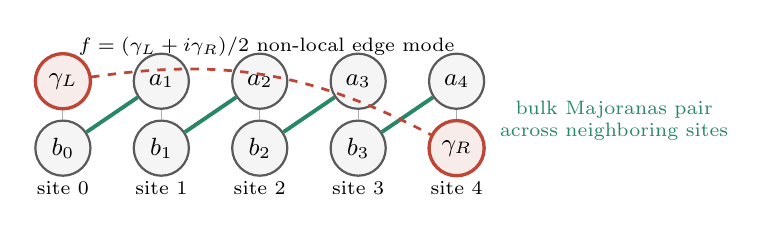
\begin{tikzpicture}[
  font=\small,
  maj/.style={circle, draw=linkgray, thick, fill=softgray, minimum size=7mm, inner sep=0pt},
  edge/.style={circle, draw=isingred, very thick, fill=isingred!10, minimum size=7mm, inner sep=0pt},
  pair/.style={line width=1.4pt, draw=kitaevgreen},
  weak/.style={dashed, line width=1.0pt, draw=isingred}
]
  \foreach \j in {0,1,2,3,4} {
    \node[maj] (a\j) at (1.25*\j,0) {$a_{\j}$};
    \node[maj] (b\j) at (1.25*\j,-0.85) {$b_{\j}$};
    \draw[linkgray!50] (a\j) -- (b\j);
    \node[font=\scriptsize] at (1.25*\j,-1.35) {site \j};
  }
  \node[edge] at (a0) {$\gamma_L$};
  \node[edge] at (b4) {$\gamma_R$};
  \foreach \j/\k in {0/1,1/2,2/3,3/4} {
    \draw[pair] (b\j) -- (a\k);
  }
  \draw[weak, bend left=18] (a0) to node[above=3pt, align=center, font=\scriptsize]
    {$f=(\gamma_L+i\gamma_R)/2$ non-local edge mode} (b4);
  \node[align=center, font=\scriptsize, kitaevgreen] at (7,-0.5)
    {bulk Majoranas pair \\ across neighboring sites};
\end{tikzpicture}
\caption{At the topological sweet spot, the bulk Majoranas pair locally while
one Majorana remains at each end. The two edge Majoranas form a non-local
fermion whose occupation labels the near-degenerate parity sectors.}
\label{fig:majorana-chain}
\end{figure}

\subsection{Jordan-Wigner qubit form}

Under the Jordan-Wigner mapping, the Hamiltonian becomes
\begin{equation}
  H_K
  =
  -\frac{\mu}{2}\sum_{j=0}^{L-1}Z_j
  +\frac{t-\Delta}{2}\sum_{j=0}^{L-2}X_jX_{j+1}
  +\frac{t+\Delta}{2}\sum_{j=0}^{L-2}Y_jY_{j+1}.
  \label{eq:kitaev-qubit}
\end{equation}
The qubit $Z_j$ has a direct fermionic meaning:
\begin{equation}
  n_j=c_j^\dagger c_j=\frac{I-Z_j}{2}.
\end{equation}
The total fermion parity is
\begin{equation}
  P=\prod_{j=0}^{L-1}Z_j.
\end{equation}
The $X_j$ and $Y_j$ operators are not simply local fermion observables; under
the inverse Jordan-Wigner map they include parity strings. This is why local
spin order in the qubit language can correspond to non-local string order in
the fermion language.

\section{Sweet Spot: Why It Looks Like an AFM Ising Chain}

At $t=\Delta$, the $XX$ term cancels:
\begin{equation}
  H_K(t=\Delta)
  =
  -\frac{\mu}{2}\sum_j Z_j
  +t\sum_{j=0}^{L-2}Y_jY_{j+1}.
\end{equation}
At $\mu=0$,
\begin{equation}
  H_K(t=\Delta,\mu=0)
  =
  t\sum_{j=0}^{L-2}Y_jY_{j+1}.
  \label{eq:pure-yy}
\end{equation}
This is algebraically the same structure as an antiferromagnetic Ising chain,
but in the $Y$ basis rather than the $Z$ basis.

If $\mu$ is turned back on, $-\mu\sum_jZ_j/2$ does not commute with the
$Y_jY_{j+1}$ ordering term. After a spin-axis rotation that sends $Y$ to $Z$,
this term plays the algebraic role of a transverse field. This is why the
qubit Hamiltonian resembles a transverse-field Ising model near the sweet spot.
The physical meaning is still different: $\mu$ is a chemical potential for
fermions, and the transition at $|\mu|=2t$ is the closing and reopening of a
topological superconducting gap.

Let $\ket{+y}$ and $\ket{-y}$ be eigenstates of $Y$:
\begin{equation}
  Y\ket{+y}=+\ket{+y},
  \qquad
  Y\ket{-y}=-\ket{-y}.
\end{equation}
In the occupation/computational basis,
\begin{equation}
  \ket{+y}=\frac{\ket{0}+i\ket{1}}{\sqrt{2}},
  \qquad
  \ket{-y}=\frac{\ket{0}-i\ket{1}}{\sqrt{2}}.
\end{equation}
So a $Y$-basis Neel state is already a coherent superposition of many fermion
occupation configurations. It should not be read as a classical pattern of
particles sitting on alternating sites.

For one bond,
\begin{equation}
  tY_jY_{j+1}
\end{equation}
has energy $+t$ when neighboring $Y$ eigenvalues are equal and energy $-t$
when they are opposite. Thus, for $t>0$, the two qubit-spin ground states of
Eq.~\eqref{eq:pure-yy} are
\begin{equation}
  \ket{\widetilde N_1}
  =
  \ket{+y,-y,+y,-y,\ldots},
  \qquad
  \ket{\widetilde N_2}
  =
  \ket{-y,+y,-y,+y,\ldots},
  \label{eq:y-neel}
\end{equation}
with energy
\begin{equation}
  E_0=-t(L-1).
\end{equation}

The parity operator $P=\prod_j Z_j$ maps these two states into each other:
\begin{equation}
  P\ket{\widetilde N_1}=\ket{\widetilde N_2},
  \qquad
  P\ket{\widetilde N_2}=\ket{\widetilde N_1}.
\end{equation}
Since $[H_K,P]=0$, one may choose definite-parity ground states instead:
\begin{equation}
  \ket{\psi_\pm}
  =
  \frac{1}{\sqrt{2}}
  \left(\ket{\widetilde N_1}\pm\ket{\widetilde N_2}\right),
  \qquad
  P\ket{\psi_\pm}=\pm\ket{\psi_\pm}.
\end{equation}
This is the first place where the interpretation changes: the same degenerate
subspace can be written as two $Y$-ordered spin states or as two fermion-parity
states. The Kitaev-chain interpretation uses the parity states and the edge
Majorana mode that connects them.

\begin{figure}[h]
\centering
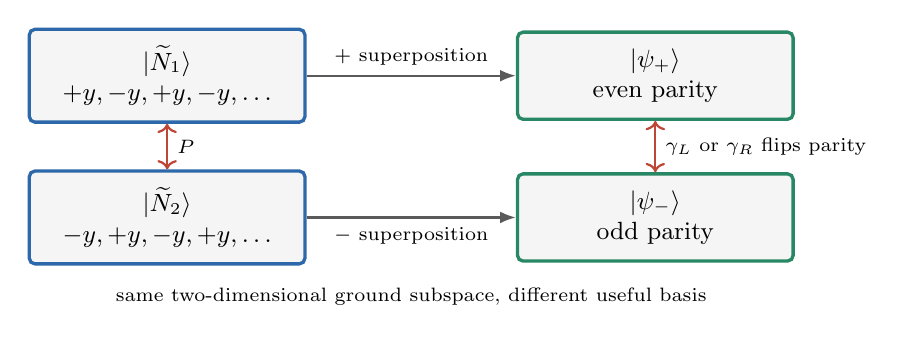
\begin{tikzpicture}[
  font=\small,
  state/.style={draw, rounded corners=2pt, fill=softgray, align=center,
    inner sep=6pt, minimum width=3.5cm, minimum height=0.95cm},
  arr/.style={-{Latex[length=2mm]}, thick, draw=linkgray}
]
  \node[state, draw=isingblue, very thick] (n1) at (0,0)
    {$\ket{\widetilde N_1}$\\ $+y,-y,+y,-y,\ldots$};
  \node[state, draw=isingblue, very thick] (n2) at (0,-1.8)
    {$\ket{\widetilde N_2}$\\ $-y,+y,-y,+y,\ldots$};
  \node[state, draw=kitaevgreen, very thick] (pplus) at (6.2,0)
    {$\ket{\psi_+}$\\ even parity};
  \node[state, draw=kitaevgreen, very thick] (pminus) at (6.2,-1.8)
    {$\ket{\psi_-}$\\ odd parity};
  \draw[arr] (n1) -- node[above, font=\scriptsize] {$+$ superposition} (pplus);
  \draw[arr] (n2) -- node[below, font=\scriptsize] {$-$ superposition} (pminus);
  \draw[<->, thick, draw=isingred] (n1) -- node[right, font=\scriptsize] {$P$} (n2);
  \draw[<->, thick, draw=isingred] (pplus) -- node[right, font=\scriptsize] {$\gamma_L$ or $\gamma_R$ flips parity} (pminus);
  \node[align=center, font=\scriptsize] at (3.1,-2.8)
    {same two-dimensional ground subspace, different useful basis};
\end{tikzpicture}
\caption{The pure $YY$ Hamiltonian has two $Y$-Neel product states, but the
Kitaev interpretation reorganizes this subspace into definite fermion-parity
states connected by edge Majorana operators.}
\label{fig:parity-basis}
\end{figure}

So, as a spin Hamiltonian, the sweet-spot Kitaev qubit Hamiltonian is an
antiferromagnetic Ising chain after rotating the spin axes from $Y$ to $Z$.
That statement is correct but incomplete.

\section{Where the Physics Diverges}

\subsection{Different degrees of freedom}

In the AFM Ising model, the spins are the physical ordered variables. Measuring
$Z_j$ locally tells us whether the system chose one staggered pattern or the
other.

In the Kitaev problem, the qubits encode fermions. The $Z_j$ operator measures
local occupation parity, but $X_j$ and $Y_j$ contain Jordan-Wigner strings in
fermion language. Therefore the $Y$-Neel order in Eq.~\eqref{eq:y-neel} is not
an ordinary local magnetic order of the original fermions. It is the spin-chain
image of superconducting/topological order.

\subsection{Different meaning of degeneracy}

For the AFM Ising chain, the two ground states are two locally distinguishable
patterns:
\begin{equation}
  \ket{\up\down\up\down\cdots}
  \quad \text{versus} \quad
  \ket{\down\up\down\up\cdots}.
\end{equation}
The degeneracy is tied to symmetry breaking. A local staggered field can select
one pattern.

For the open Kitaev chain in the topological phase, the degeneracy is tied to
Majorana edge modes. The two edge Majoranas combine into a non-local fermionic
mode
\begin{equation}
  f=\frac{1}{2}(\gamma_L+i\gamma_R).
\end{equation}
The two low-energy states differ by whether this non-local fermion is empty or
occupied:
\begin{equation}
  n_f=f^\dagger f=0 \quad \text{or} \quad 1.
\end{equation}
Changing $n_f$ flips total fermion parity. A local parity-preserving fermion
operator cannot directly change this edge occupation, because that would require
coupling the two ends of the chain. In a finite chain away from the exact sweet
spot, the splitting between the two parity sectors is exponentially small in
system size:
\begin{equation}
  |E_0^{(+)}-E_0^{(-)}|\sim e^{-L/\xi}.
\end{equation}
This is the Majorana hybridization splitting, not the energy cost of a local
spin-domain-wall defect.

\subsection{Different symmetry story}

The AFM Ising Hamiltonian has a global spin-flip symmetry, and the ordered
phase breaks that symmetry by selecting one Neel pattern. When translation is a
symmetry, the same order also breaks one-site translation down to two-site
translation. The order parameter is local:
\begin{equation}
  m_{\mathrm{stag}}=\frac{1}{L}\sum_j(-1)^jZ_j.
\end{equation}

The Kitaev chain has conserved fermion parity:
\begin{equation}
  [H_K,P]=0.
\end{equation}
The topological phase does not require a local order parameter that breaks
fermion parity. In fact, operators corresponding to a single Majorana edge mode
flip parity, so their expectation value vanishes in a parity eigenstate. The
robust diagnostic is parity-preserving and non-local, for example
\begin{equation}
  O_{\mathrm{edge}}
  =
  X_0Z_1\cdots Z_{L-2}X_{L-1}.
\end{equation}
For $L=4$,
\begin{equation}
  O_{\mathrm{edge}}=X_0Z_1Z_2X_3.
\end{equation}
This is why Week 5 and Week 6 focus on string/correlation observables rather
than local magnetization.

\begin{figure}[h]
\centering
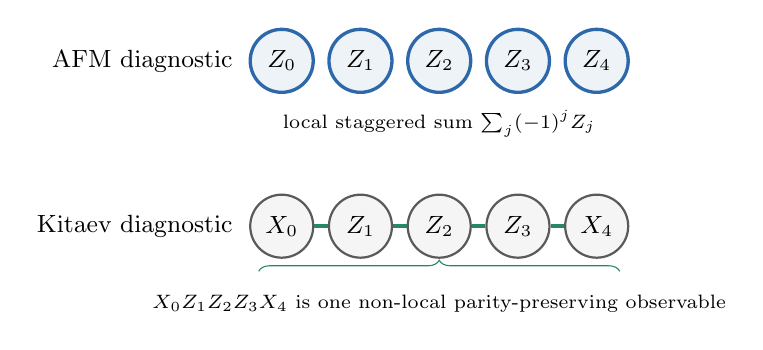
\begin{tikzpicture}[
  font=\small,
  site/.style={circle, draw=linkgray, thick, fill=softgray, minimum size=8mm, inner sep=0pt},
  local/.style={site, draw=isingblue, very thick, fill=isingblue!8},
  string/.style={line width=1.4pt, draw=kitaevgreen}
]
  \node[anchor=east] at (-0.5,0) {AFM diagnostic};
  \foreach \i/\lab in {0/{Z_0},1/{Z_1},2/{Z_2},3/{Z_3},4/{Z_4}} {
    \node[local] (s\i) at (\i*1.0,0) {$\lab$};
  }
  \node[font=\scriptsize, align=center] at (2,-0.8)
    {local staggered sum $\sum_j(-1)^jZ_j$};

  \node[anchor=east] at (-0.5,-2.1) {Kitaev diagnostic};
  \foreach \i/\lab in {0/{X_0},1/{Z_1},2/{Z_2},3/{Z_3},4/{X_4}} {
    \node[site] (k\i) at (\i*1.0,-2.1) {$\lab$};
  }
  \draw[string] (k0.east) -- (k1.west);
  \draw[string] (k1.east) -- (k2.west);
  \draw[string] (k2.east) -- (k3.west);
  \draw[string] (k3.east) -- (k4.west);
  \draw[decorate, decoration={brace, amplitude=4pt}, draw=kitaevgreen]
    ($(k0.south west)+(0,-0.28)$) -- node[below=5pt, font=\scriptsize]
    {$X_0Z_1Z_2Z_3X_4$ is one non-local parity-preserving observable}
    ($(k4.south east)+(0,-0.28)$);
\end{tikzpicture}
\caption{The Ising order parameter is a sum of local measurements. The Kitaev
edge diagnostic is a single non-local string that ties the two ends together
while preserving total fermion parity.}
\label{fig:local-vs-string}
\end{figure}

\subsection{Different protection mechanism}

AFM order is stable because a local domain wall costs finite energy. However,
the two ordered patterns are locally distinguishable, and a local staggered
field directly favors one over the other.

The Kitaev topological degeneracy is protected differently. The two Majoranas
live at opposite ends of an open chain, so a local parity-preserving
perturbation cannot easily couple them. The splitting is controlled by the
overlap of edge-mode wavefunctions and is exponentially small in $L$. This is a
non-local protection mechanism, not ordinary local symmetry breaking.

\section{Comparison Table}

\begin{center}
\small
\begin{tabular}{p{0.23\linewidth}p{0.33\linewidth}p{0.35\linewidth}}
\toprule
Feature & AFM Ising chain & Kitaev-chain qubit Hamiltonian \\
\midrule
Simple Hamiltonian
& $J\sum Z_jZ_{j+1}$, $J>0$
& $t\sum Y_jY_{j+1}$ at $t=\Delta,\mu=0$ \\[3pt]
Low-energy bond
& opposite $Z$ eigenvalues
& opposite $Y$ eigenvalues \\[3pt]
Ground states
& two $Z$-basis Neel states
& two $Y$-basis Neel-like qubit states at the sweet spot \\[3pt]
Physical variables
& spins are the ordered variables
& qubits encode fermions via Jordan-Wigner \\[3pt]
Degeneracy source
& broken discrete spin symmetry
& Majorana edge mode / fermion parity sectors \\[3pt]
Order parameter
& local staggered magnetization
& non-local string / edge correlation in fermion language \\[3pt]
Excitations
& local domain walls
& bulk quasiparticles plus edge-mode parity splitting \\[3pt]
Protection
& local energy cost for bad bonds
& exponentially weak edge-edge coupling in an open chain \\
\bottomrule
\end{tabular}
\end{center}

\section{Takeaway}

The sweet-spot Kitaev qubit Hamiltonian and an AFM Ising chain can have the
same algebraic form after a spin-basis rotation:
\begin{equation}
  J\sum Z_jZ_{j+1}
  \quad \leftrightarrow \quad
  t\sum Y_jY_{j+1}.
\end{equation}
But they answer different physical questions. The AFM Ising model describes
local staggered spin order and symmetry breaking. The Kitaev chain describes a
topological superconducting phase whose qubit Hamiltonian only looks like a
spin model after Jordan-Wigner encoding. Its key signatures are conserved
fermion parity, Majorana edge modes, exponentially small parity splitting, and
non-local string correlations.

\end{document}
